
Esta secci\'on agrupa las herramientas t\'ecnicas que sustentan las distribuciones
muestrales. Las distribuciones que aqu\'i se estudian (Z, t, $\chi^2$, F) son la
columna vertebral de la inferencia estad\'istica cl\'asica y aparecen de manera
recurrente en problemas de ciencia de datos.


\section{Transformación de variables}

Una pregunta frecuente en estad\'istica es: si $X$ tiene una distribuci\'on conocida
y definimos $Y = g(X)$ para alguna funci\'on $g$, ¿cu\'al es la distribuci\'on de $Y$?

\subsection{Transformaci\'on lineal}

\begin{teorema}[Transformaci\'on af\'in]
Si $X$ es una variable aleatoria con media $\mu_X$ y varianza $\sigma_X^2$, y
$Y = aX + b$ con $a \neq 0$, entonces
\begin{align}
 \label{eq:3.2.1}
 \mu_Y &= a\mu_X + b, \\
 \label{eq:3.2.2}
 \sigma_Y^2 &= a^2\sigma_X^2.
\end{align}
Adem\'as, si $X$ tiene funci\'on de distribuci\'on $F_X$, entonces
$F_Y(y) = F_X\!\left(\frac{y-b}{a}\right)$.
\end{teorema}

\begin{ejemplo}
 \label{exmp:3.2.1}
Si $X \sim N(\mu, \sigma^2)$ y $Y = aX + b$ con $a \neq 0$, entonces
$Y \sim N(a\mu + b, a^2\sigma^2)$. Esta es la \emph{propiedad de reproductividad}
de la distribuci\'on normal bajo transformaciones lineales.
\end{ejemplo}

\subsection{Teorema de cambio de variable}

Para transformaciones m\'as generales, necesitamos el siguiente resultado.

\begin{teorema}[Cambio de variable, caso mon\'otono]
Sean $X$ una variable aleatoria continua con densidad $f_X$, y $g$ una funci\'on
estrictamente mon\'otona y diferenciable. Si $Y = g(X)$ y $g^{-1}$ denota la inversa
de $g$, entonces la densidad de $Y$ es
\begin{align}
 \label{eq:3.2.3}
 f_Y(y) = f_X\!\left(g^{-1}(y)\right) \cdot \left|\frac{d}{dy}\,g^{-1}(y)\right|,
\end{align}
para todo $y$ en el rango de $g$.
\end{teorema}

\begin{proof}
Supongamos $g$ creciente. Para $y$ en el rango de $g$,
\begin{align}
 F_Y(y) = P(Y \leq y) = P(g(X) \leq y) = P(X \leq g^{-1}(y)) = F_X(g^{-1}(y)).
\end{align}
Derivando y aplicando la regla de la cadena,
\begin{align}
 f_Y(y) = \frac{d}{dy} F_X(g^{-1}(y)) = f_X(g^{-1}(y)) \cdot \frac{d}{dy} g^{-1}(y).
\end{align}
El caso $g$ decreciente es an\'alogo, tomando valor absoluto.
\end{proof}

\begin{observacion}[Forma alternativa]
Si escribimos $x = g^{-1}(y)$ y denotamos $J(y) = \frac{dx}{dy}$ el Jacobiano de la
transformaci\'on inversa, la f\'ormula se reescribe como
\begin{align}
 \label{eq:3.2.4}
 f_Y(y) = f_X(x)\,|J(y)|, \quad \text{donde } x = g^{-1}(y).
\end{align}
En dimensi\'on superior, $|J(y)|$ es el valor absoluto del determinante Jacobiano.
\end{observacion}

\begin{ejemplo}
 \label{exmp:3.2.2}
Sea $X \sim \text{Exp}(1)$ con densidad $f_X(x) = e^{-x}$ para $x > 0$. Encuentre la
distribuci\'on de $Y = e^X$.
\end{ejemplo}

\begin{solucion}
La transformaci\'on $g(x) = e^x$ es estrictamente creciente de $(0, \infty)$ a
$(1, \infty)$, con inversa $g^{-1}(y) = \ln y$. Adem\'as, $\frac{d}{dy}\ln y = 1/y$.

Por el teorema de cambio de variable, para $y > 1$:
\begin{align}
 f_Y(y) = f_X(\ln y) \cdot \frac{1}{y} = e^{-\ln y} \cdot \frac{1}{y} = \frac{1}{y} \cdot \frac{1}{y} = \frac{1}{y^2}.
\end{align}

Por lo tanto, $Y$ tiene densidad $f_Y(y) = 1/y^2$ para $y > 1$ (una distribuci\'on
de Pareto con par\'ametro $\alpha = 1$).
\end{solucion}

\begin{ejemplo}
 \label{exmp:3.2.3}
Sea $X \sim N(\mu, \sigma^2)$. Encuentre la distribuci\'on de $Y = e^X$ (la
distribuci\'on \emph{log-normal}).
\end{ejemplo}

\begin{solucion}
La transformaci\'on $g(x) = e^x$ es creciente, con inversa $g^{-1}(y) = \ln y$.
La densidad de $X$ es
\begin{align}
 f_X(x) = \frac{1}{\sigma\sqrt{2\pi}}\,\exp\!\left(-\frac{(x-\mu)^2}{2\sigma^2}\right).
\end{align}

Aplicando el teorema, para $y > 0$:
\begin{align}
 f_Y(y) &= f_X(\ln y) \cdot \frac{1}{y} \\
 &= \frac{1}{\sigma\sqrt{2\pi}}\,\exp\!\left(-\frac{(\ln y - \mu)^2}{2\sigma^2}\right) \cdot \frac{1}{y}.
\end{align}

Por lo tanto, $Y$ sigue una distribuci\'on log-normal $LN(\mu, \sigma^2)$.
\end{solucion}

\begin{ejemplo}
 \label{exmp:3.2.4}
Sea $X \sim U(0, 2\pi)$ uniforme. Encuentre la distribuci\'on de $Y = \sin(X)$ (caso
no mon\'otono).
\end{ejemplo}

\begin{solucion}
La funci\'on $g(x) = \sin x$ no es mon\'otona en $(0, 2\pi)$: alcanza el m\'aximo
$1$ en $x = \pi/2$ y el m\'inimo $-1$ en $x = 3\pi/2$. Cada valor $y \in (-1, 1)$
tiene dos preim\'agenes: $x_1 = \arcsin y$ y $x_2 = \pi - \arcsin y$.

Usando la f\'ormula para el caso no mon\'otono,
\begin{align}
 f_Y(y) &= \sum_{x: \sin x = y} f_X(x) \cdot \left|\frac{dx}{dy}\right| \\
 &= \frac{1}{2\pi}\cdot\frac{1}{\sqrt{1-y^2}} + \frac{1}{2\pi}\cdot\frac{1}{\sqrt{1-y^2}} \\
 &= \frac{1}{\pi\sqrt{1-y^2}}, \quad y \in (-1, 1).
\end{align}

Esta es la densidad del \emph{arcoseno}, que aparece en el \emph{camino aleatorio}.
\end{solucion}

\subsection{Transformaciones comunes}

\begin{observacion}
Las siguientes transformaciones son \'utiles para \emph{normalizar} datos o
estabilizar varianzas:
\begin{itemize}
 \item $Y = \ln X$: comprime valores grandes, expande valores cercanos a $0$.
 \item $Y = \sqrt{X}$: suaviza la asimetr\'ia de conteos.
 \item $Y = X^{1/3}$: alternativa a la ra\'iz cuadrada para datos con asimetr\'ia
 pronunciada.
 \item \emph{Box-Cox}: $Y = (X^\lambda - 1)/\lambda$ para $\lambda \neq 0$;
 $Y = \ln X$ para $\lambda = 0$. Optimiza la normalidad.
\end{itemize}
\end{observacion}

\lstinputlisting[language=Python]{../code/distribuciones-muestreo/transformacionesVariables.py}

\begin{figure}
 \centering
 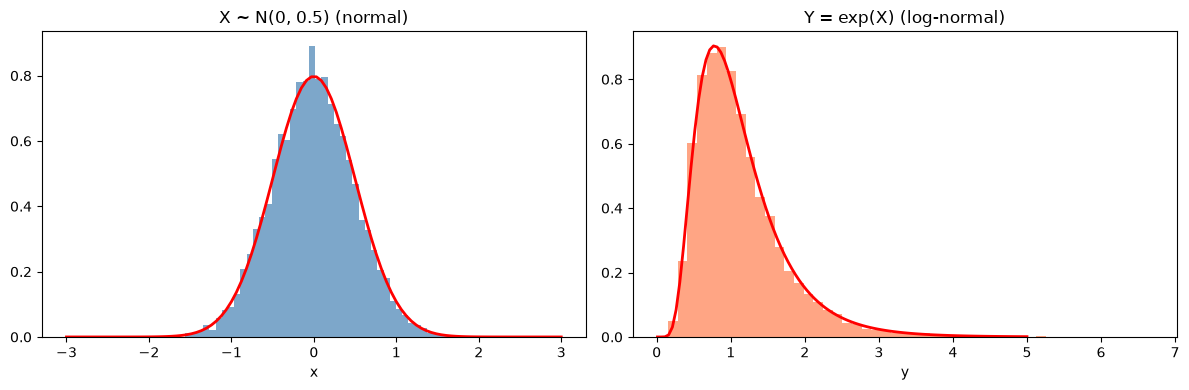
\includegraphics[height=7cm,keepaspectratio=true]{./pe/transformaciones.png}
 % transformaciones.png: 0x0 pixel, 300dpi, 0.00x0.00 cm, bb=
 \caption{Transformaci\'on exponencial: de normal a log-normal.}
 \label{fig:3.2.1}
\end{figure}


